\clearpage
\VerdierPhysicalPageAnchor{0103}%
\begingroup
\small
\setlength{\abovedisplayskip}{3pt plus 2pt minus 2pt}%
\setlength{\belowdisplayskip}{3pt plus 2pt minus 2pt}%
\setlength{\jot}{2pt}%

\VerdierSemanticAnchor{ch1-3-4-2-variable-specialization}
Let $j\in[n]$, and for every $i\neq j$ let $X_i$ be an object of $K(C_i)$.
Denote by
\[
  G\colon K(C_j)\longrightarrow K(C)
\]
the functor

\VerdierSemanticAnchor{ch1-3-4-2-1}
\begingroup
\makeatletter
\tagsleft@true
\let\veqno\@@leqno
\makeatother
\begin{equation}
  X\longmapsto G(X)=K_{\Pi}F(X_1,\ldots,X,\ldots,X_n),
  \tag{3.4.2.1}
\end{equation}
\endgroup
\VerdierSemanticAnchor{ch1-3-4-2-translation-isomorphism}
and by
\[
  m\colon G(X[1])\xrightarrow{\sim}G(X)[1]
\]
the functorial isomorphism deduced from $p_j$.

\VerdierSemanticAnchor{ch1-3-4-3}
\noindent\textbf{Proposition 3.4.3.}\quad
\emph{For every distinguished triangle}
\VerdierSemanticAnchor{ch1-3-4-3-input-triangle}
\[
  X\xrightarrow{u}Y\xrightarrow{v}Z\xrightarrow{w}X[1]
\]
\emph{in $K(C_j)$, the triangle in $K(C)$}
\VerdierSemanticAnchor{ch1-3-4-3-image-triangle}
\[
  G(X)\xrightarrow{G(u)}G(Y)\xrightarrow{G(v)}G(Z)
  \xrightarrow{mG(w)}G(X)[1]
\]
\emph{is distinguished.}

\VerdierSemanticAnchor{ch1-3-4-3-proof}
We may first suppose that the distinguished triangle in $K(C_j)$ has the
form (3.3.1):
\VerdierSemanticAnchor{ch1-3-4-3-cone-model}
\[
  X\xrightarrow{\dot f}Y\xrightarrow{\dot p(f)}c(f)
  \xrightarrow{\dot q(f)}X[1],
\]
where $f\colon X\longrightarrow Y$ is a morphism in
$\operatorname{comp}(C_j)$. Denote by
\VerdierSemanticAnchor{ch1-3-4-3-complex-functor}
\[
  H\colon\operatorname{comp}(C_j)\longrightarrow\operatorname{comp}(C)
\]
the functor
\[
  X\longmapsto H(X)=\operatorname{comp}_{\Pi}F
  (X_1,\ldots,X,\ldots,X_n),
\]
\VerdierSemanticAnchor{ch1-3-4-3-complex-translation-isomorphism}
and by
\[
  m\colon H(X[1])\xrightarrow{\sim}H(X)[1]
\]
the functorial isomorphism commuting with translations in direction $j$.
The functor $(G,m)$ is obtained from the functor $(H,m)$ by passing to
complexes up to homotopy. To prove the proposition, it suffices to show that
there is an isomorphism of complexes in $\operatorname{comp}(C)$

\VerdierSemanticAnchor{ch1-3-4-3-cone-isomorphism}
\[
  J\colon H(c(f))\xrightarrow{\sim}c(H(f))
\]
such that the following diagram is commutative:

\VerdierSemanticAnchor{ch1-3-4-3-1}
\begin{equation}
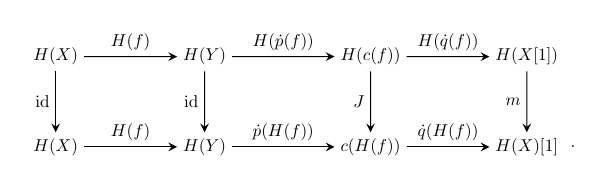
\begin{tikzpicture}[>=stealth,scale=0.62,every node/.style={transform shape}]
  \node (x1) at (0,1.85) {$H(X)$};
  \node (y1) at (3.05,1.85) {$H(Y)$};
  \node (c1) at (6.45,1.85) {$H(c(f))$};
  \node (s1) at (9.65,1.85) {$H(X[1])$};
  \node (x2) at (0,0) {$H(X)$};
  \node (y2) at (3.05,0) {$H(Y)$};
  \node (c2) at (6.45,0) {$c(H(f))$};
  \node (s2) at (9.65,0) {$H(X)[1]$};
  \draw[->] (x1) -- node[above] {$H(f)$} (y1);
  \draw[->] (y1) -- node[above] {$H(\dot p(f))$} (c1);
  \draw[->] (c1) -- node[above] {$H(\dot q(f))$} (s1);
  \draw[->] (x2) -- node[above] {$H(f)$} (y2);
  \draw[->] (y2) -- node[above] {$\dot p(H(f))$} (c2);
  \draw[->] (c2) -- node[above] {$\dot q(H(f))$} (s2);
  \draw[->] (x1) -- node[left] {$\mathrm{id}$} (x2);
  \draw[->] (y1) -- node[left] {$\mathrm{id}$} (y2);
  \draw[->] (c1) -- node[left] {$J$} (c2);
  \draw[->] (s1) -- node[left] {$m$} (s2);
  \node[anchor=west,inner sep=0pt] at ([xshift=0.35em]s2.east) {$.$};
\end{tikzpicture}
\tag{3.4.3.1}
\end{equation}
\endgroup
